\documentclass{standalone}
\usepackage{tikz,pgfplots}
\usetikzlibrary{calc}

\pgfplotsset{%
    compat=newest, %footnotesize
    tick label style={font=\footnotesize},
    label style={font=\small},
    legend style={font=\small},
    axis x line = center,
    axis y line = center,
    every axis/.style={pin distance=1ex}
    cmhplot/.style={color=black,mark=none,line width=1pt,->},
    soldot/.style={color=black,only marks,mark=*},
    coldot/.style={color=black,fill=white,only marks,mark=*},
}


\begin{document}
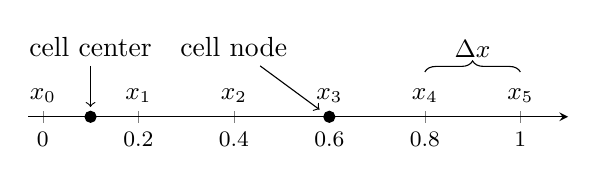
\begin{tikzpicture}
\begin{axis}[%
axis x line=center,
axis y line=none,ymin=0,ymax=1,
xmin=-0.03,xmax=1.1,
]
\node[black,above] at (axis cs:0.0,0.01){\small{$x_0$}};
\node[black,above] at (axis cs:0.2,0.01){\small{$x_1$}};
\node[black,above] at (axis cs:0.4,0.01){\small{$x_2$}};
\node[black,above] at (axis cs:0.6,0.01){\small{$x_3$}};
\node[black,above] at (axis cs:0.8,0.01){\small{$x_4$}};
\node[black,above] at (axis cs:1.0,0.01){\small{$x_5$}};
\node[black,above] at (axis cs:0.9,0.11){\small{$\Delta x$}};

\addplot[soldot]coordinates{(0.1,0.0)};
\addplot[soldot]coordinates{(0.6,0.0)};

\draw [decorate,decoration={brace,amplitude=4pt}]
(0.8,0.1)--(1.0,0.1) node[midway, above, font=\footnotesize, xshift=2pt] {};

\node[anchor=north] (source) at (axis cs:0.1,0.2){cell center};
       \node (destination) at (axis cs:0.1,0.0){};
       \draw[->](source)--(destination);

\node[anchor=north] (source) at (axis cs:0.4,0.2){cell node};
       \node (destination) at (axis cs:0.6,0.0){};
       \draw[->](source)--(destination);


\end{axis}

\end{tikzpicture}


\end{document}